\documentclass[a4paper,11pt]{jsarticle}


% 数式
\usepackage{amsmath,amsfonts,amssymb}
\usepackage{bm}
% 画像
\usepackage[dvipdfmx]{graphicx}
\usepackage[dvipdfmx]{color}
\usepackage{siunitx}
\usepackage{wrapfig}
\usepackage{cases}
\usepackage{dcolumn}
\makeatletter
\newcommand{\figsubcaption}[1]{\def\@captype{figure}\subcaption{#1}}
\newcommand{\tblsubcaption}[1]{\def\@captype{table}\subcaption{#1}}
\makeatother

% サブキャプション
\usepackage{subcaption}

\usepackage{listings,jvlisting}
\lstset{
basicstyle={\ttfamily},
identifierstyle={\small},
commentstyle={\smallitshape},
keywordstyle={\small\bfseries},
ndkeywordstyle={\small},
stringstyle={\small\ttfamily},
frame={tb},
breaklines=true,
columns=[l]{fullflexible},
numbers=left,
xrightmargin=0zw,
xleftmargin=3zw,
numberstyle={\scriptsize},
stepnumber=1,
numbersep=1zw,
lineskip=-0.5ex
}

\begin{document}

\title{2重振り子を長さと慣性モーメントが時間変化する単振り子としてみる}
\author{平林広}
\date{\today}
\maketitle


\begin{figure}[h]
  \centering
  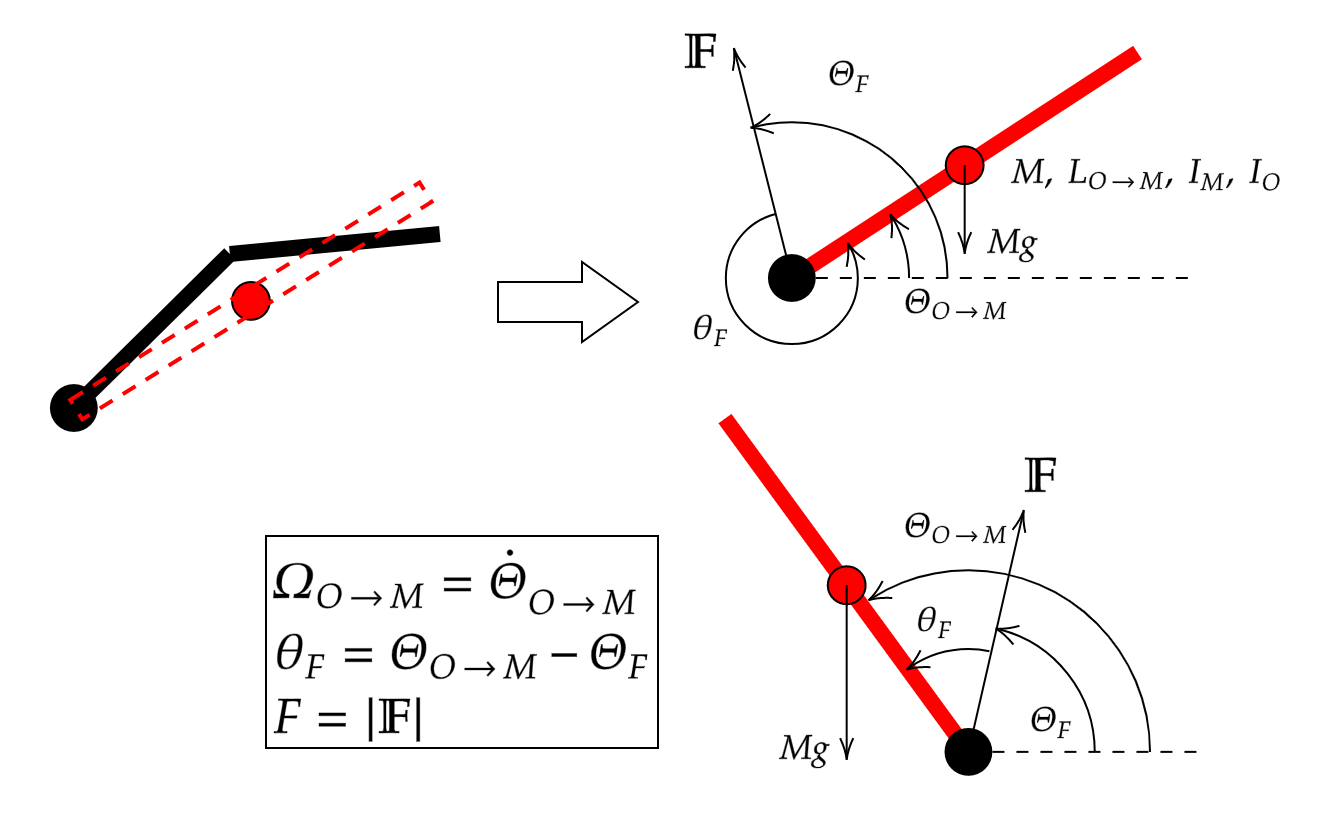
\includegraphics[width = 0.8\textwidth]{config.png}
  \caption{変数設定}
  \label{config.png}
\end{figure}

ニュートンの運動方程式は
動径方向、
固定点周りの角運動量変化$(\dot{I_O\Omega_M})$、
重心周りの角運動量変化$(\dot{I_M\Omega_M})$について成り立つ。
\begin{gather*}
  \begin{cases}
    ML_M{\Omega_M}^2 - M\ddot{L}_M = Mg\sin\Theta_M - F\cos\theta_F
    \\
    \dot{I}_O \Omega_M + I_O \dot{\Omega}_M = -Mg\cos\Theta_M L_M
    \\
    \dot{I}_M \Omega_M + I_M \dot{\Omega}_M = F\sin\theta_F
  \end{cases}
\end{gather*}

\begin{figure}[h]
  \begin{tabular}{ccccc}
    \begin{minipage}[t]{0.19\textwidth}
      \centering
      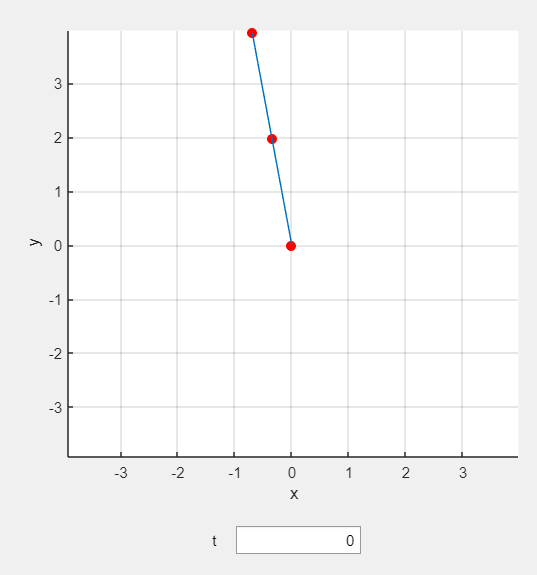
\includegraphics[width=1\textwidth]{2seg_movement_01.png}
      \subcaption{$t=0$}
    \end{minipage} &
    \begin{minipage}[t]{0.19\textwidth}
      \centering
      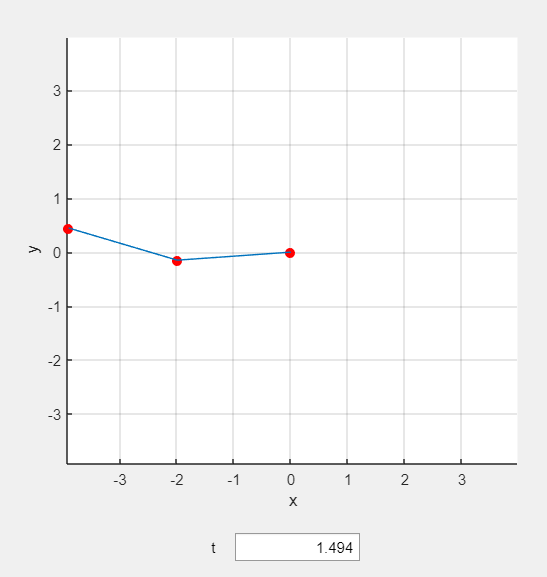
\includegraphics[width=1\textwidth]{2seg_movement_02.png}
      \subcaption{$t=1.494$}
    \end{minipage} &
    \begin{minipage}[t]{0.19\textwidth}
      \centering
      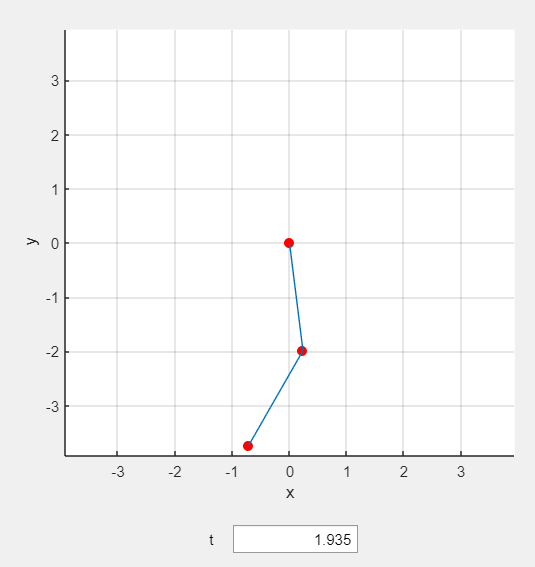
\includegraphics[width=1\textwidth]{2seg_movement_03.png}
      \subcaption{$t=1.907$}
    \end{minipage} &
    \begin{minipage}[t]{0.19\textwidth}
      \centering
      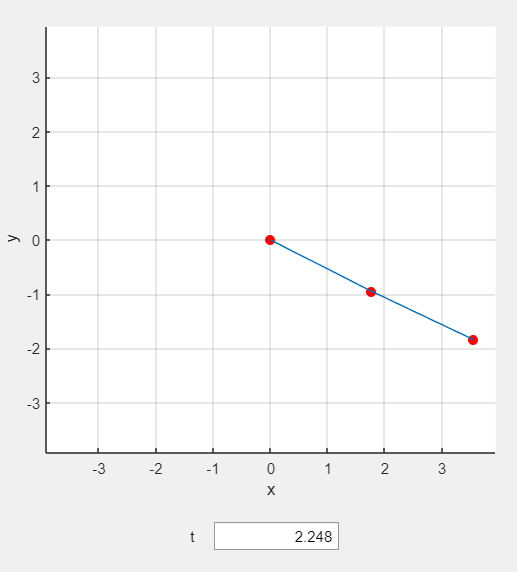
\includegraphics[width=1\textwidth]{2seg_movement_04.png}
      \subcaption{$t=2.134$}
    \end{minipage} &
    \begin{minipage}[t]{0.19\textwidth}
      \centering
      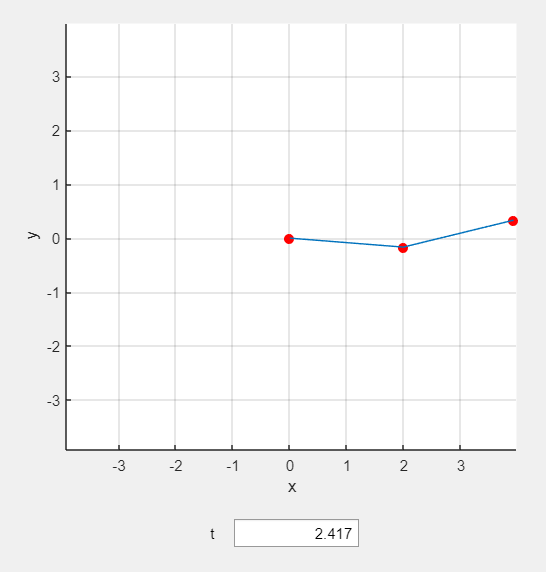
\includegraphics[width=1\textwidth]{2seg_movement_05.png}
      \subcaption{$t=2.417$}
    \end{minipage}
  \end{tabular}
  \caption{
    1セグメント目が真下になるまで
    2セグメント目が負に一定の加速度を持つようなトルクを発生させ、
    1セグメント目が真下以降は
    2セグメント目が正に一定の加速度を持つようなトルクを発生させた
    2重振り子の様子。
  }
  \label{2seg_example}
\end{figure}

図\ref{2seg_example}のような2重振り子に適用して、両辺を計算してみる.
すると
動径方向と固定点周りの角運動量変化$(\dot{I_O\Omega_M})$
に関する方程式は成り立つことが分かるが、
重心周りの角運動量変化$(\dot{I_M\Omega_M})$に関しては成り立たないことが分かる。
途中までは一致しているように見えるが、それはセグメント間のトルクが小さいためそう見えるだけである。
数値的に重心周りの角運動量を計算し、その微分をとると、それは右辺と一致することが分かる。
\begin{figure}[h]
  \centering
  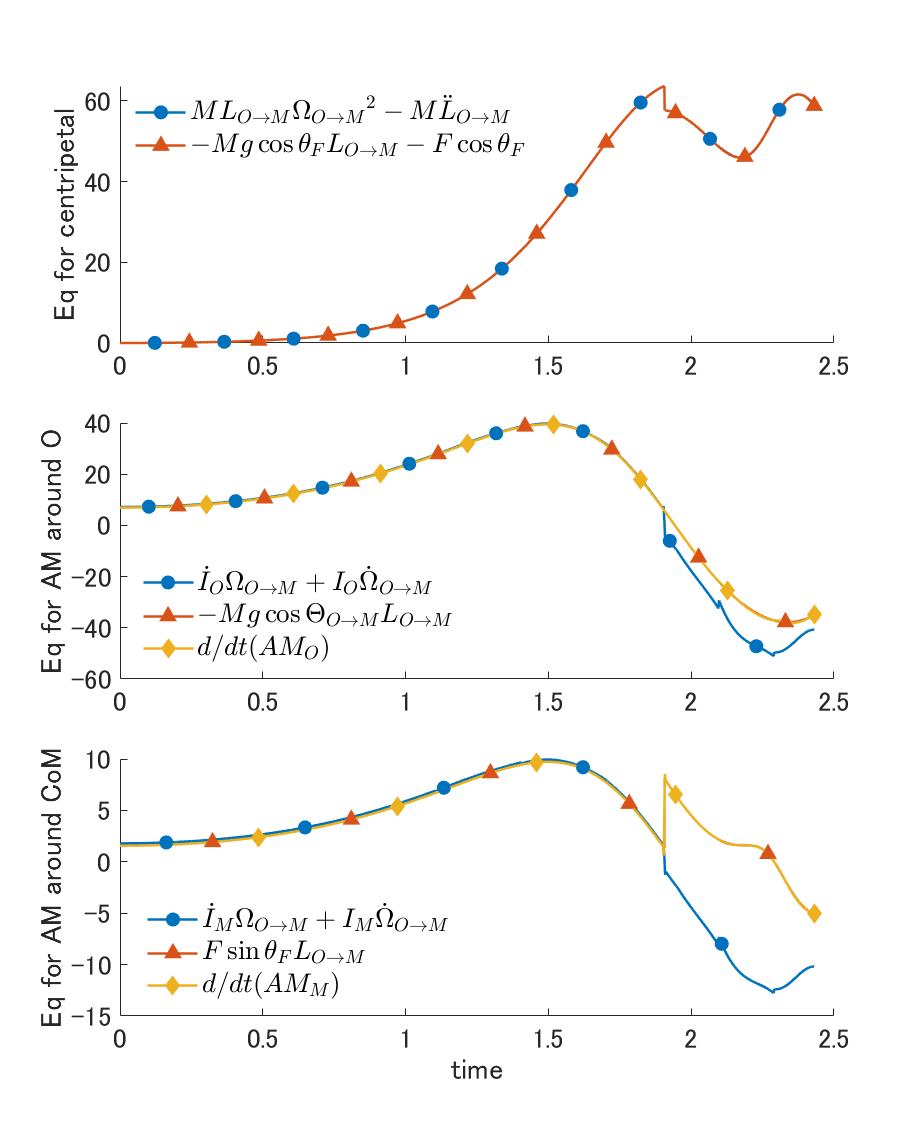
\includegraphics[width = 0.6\textwidth]{equation_values.png}
  \caption{
    各方程式の左辺と右辺の値。
    $AM$は2重振り子としての全体の重心周りの角運動量。
  }
  \label{equation_values.png}
\end{figure}

\end{document}